\documentclass[]{beamer}
\usetheme{Singapore}
\usepackage{hyperref}
\usepackage{helvet}
\usepackage{graphicx}
\usepackage{array}
\usepackage{tipa}
\usepackage{booktabs}
\usepackage[small,nohug,heads=vee]{diagrams}
\usepackage[normalem]{ulem}
\usepackage{multirow}

\mode<presentation>
\title{Using Speech Community Data as Phonological Evidence}
\author{Josef Fruehwald}
\institute{University of Pennsylvania}
\date{September 16, 2011\\Penn State, The Center for Language Science}



\AtBeginSection[]
{
  \begin{frame}<beamer>{Outline}
    \tableofcontents[currentsection]
  \end{frame}
}



\usepackage{Sweave}
\begin{document}
\begin{frame}
	\titlepage
\end{frame}

\section{Introduction}

\subsection{Motivations}

\begin{frame}
	\frametitle{Motivations}
	\framesubtitle{Phonological Context}
	
	\begin{block}{``Classic'' Evidence}
		\begin{itemize}
			\item Alternations / Static Distributions.
			\item Drawn from introspection / Small number of informants.
		\end{itemize}
	\end{block}
	
	\begin{block}{LabPhon}
		\begin{itemize}
			\item Experimental Measures (acoustic, articulatory, judgments).
			\item Drawn from standard pools of experimental subjects.
			\item Frequently expressing concerns about the validity of Classic phonological evidence.
		\end{itemize}
	\end{block}
	
\end{frame}

\begin{frame}
	\frametitle{Motivations}
	\framesubtitle{Sociolinguistic Context}
	
	\begin{block}{Linguistic Theory}
		\begin{itemize}
			\item Variable Rules
			\item Lexical Phonology (Guy, 1991a;b)
			\item Exemplar Theory
		\end{itemize}
	\end{block}
	
	\begin{block}{Variation Theory}
		\begin{itemize}
			\item What is changing where, and how?
			\item What can influence variation?
		\end{itemize}
	\end{block}
	
	\begin{block}{Social Theory}
		\begin{itemize}
			\item How does one construct and project their identity?
		\end{itemize}
	\end{block}
\end{frame}

\begin{frame}
	\frametitle{Motivations}
	\framesubtitle{Sociolinguistic Context}
	\begin{block}{Research Focus of Papers in the Proceedings of NWAV}
		\begin{center}
		\begin{tabular}{rrrrr}
			\toprule
						&Linguistic & Variation & Social & Etc.\\
			\cmidrule{2-5}
			NWAV 37 &      2         &   8       &   4       & --      \\
			NWAV 38 &     1          &     12 &    4     &   2   \\
			\bottomrule
		\end{tabular}
		\end{center}
	\end{block}
\end{frame}

\begin{frame}
	\frametitle{Motivations}
	\framesubtitle{Using Variation for Phonological Argument}
	
	\begin{block}{Andries Coetzee}
		\begin{itemize}
			\item [$\sim$] Frequency biases in phonological variation, {\it NLLT} (w/ Shigeto Kawahara)
			\item [$\sim$] The place of variation in phonological theory, {\it The Handbook of Phonological Theory. 2nd Edition} (w/ Joe Pater)
			\item [$\sim$] \ldots
		\end{itemize}	
	\end{block}
	
	\begin{block}{Ricardo Berm\'udez-Otero}
		\begin{itemize}
			\item [$\sim$] Cycles and continua: on unidirectionality and gradualness in language change {\it Handbook on the history of English} (w/ Graeme Trousdale)
			\item [2007] Diachronic phonology {\it The Cambridge handbook of phonology}
			\item [$\sim$] \ldots
		\end{itemize}
	\end{block}
\end{frame}


\subsection{Goals}

\begin{frame}
	\frametitle{Goals}
	
	\begin{itemize}
		\item Identify how sociolinguistic data can be used for phonological theory building.
		\item Identify how sociolinguistic data can be used for identifying and specifying phonological phenomena.
		\item Identify the ways in which sociolinguistic data achieves these goals uniquely.
	\end{itemize}

\end{frame}

\subsection{Data}

\begin{frame}{Data Sources}

	\begin{block}{Philadelphia Corpus}
		Automatically extracted vowel measurements from 272 Philadelphia speakers interviewed between 1973 and 2010. Dates of birth
		ranging from 1888 to 1991.
	\end{block}
	
	\begin{block}{Atlas of North American English}
		Acoustic vowel measurements from survey respondents in the Atlas of North American English.
	\end{block}

	\begin{block}{Sociolinguistic Literature}
		Various accounts of sound change in progress from the sociolinguistic literature.
	\end{block}



\end{frame}

\begin{frame}{Philadelphia Corpus}
	\framesubtitle{FAAV Project}
%	\begin{columns}[c]
	
%	\column{1.5in}
	\begin{diagram}
		\raisebox{-.5\height}{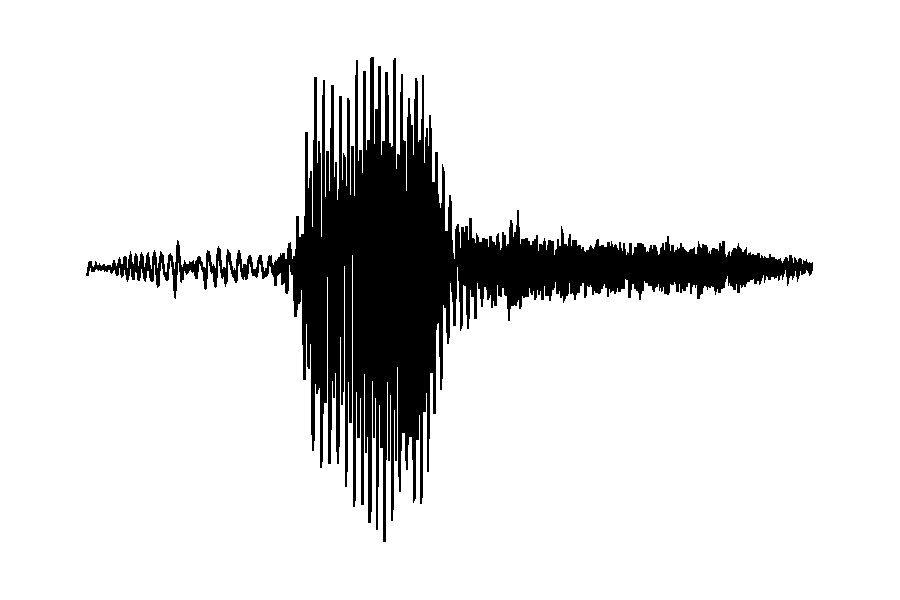
\includegraphics[width = 0.1\textwidth]{figures/wav.pdf}} &&
		\raisebox{-.5\height}{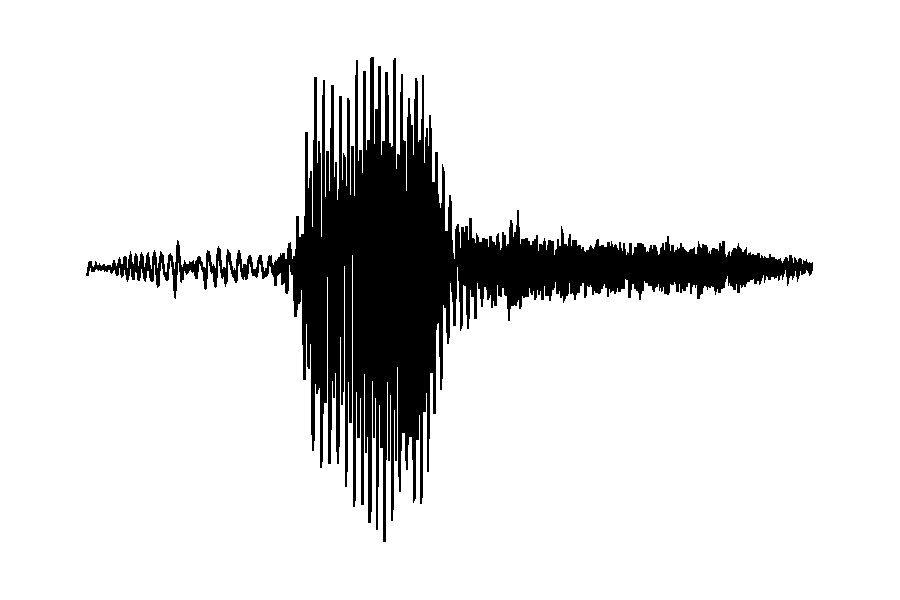
\includegraphics[width = 0.1\textwidth]{figures/wav.pdf}} + \fbox{transcription} &&
		\raisebox{-.5\height}{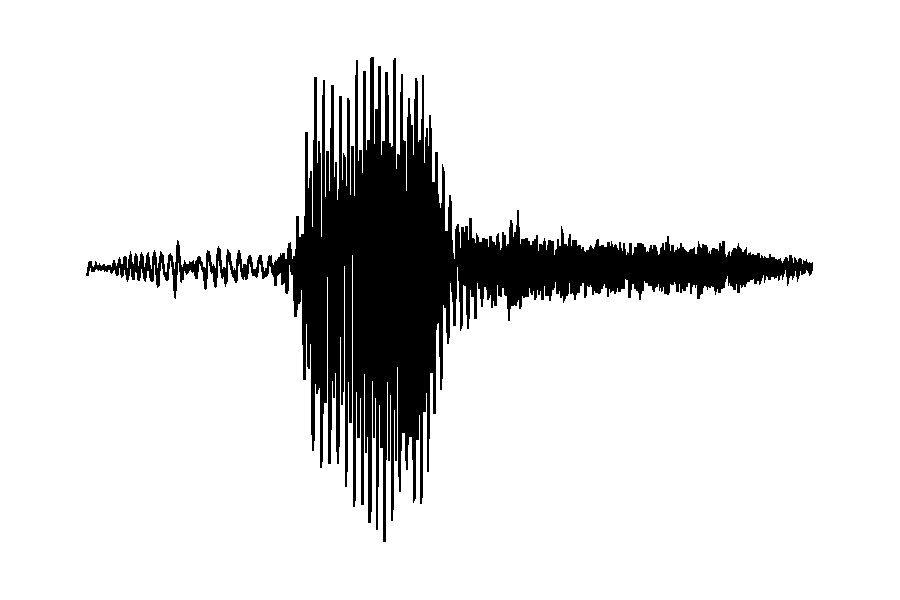
\includegraphics[width = 0.1\textwidth]{figures/wav.pdf}} + \fbox{forced\vphantom{g}}\fbox{alignment}\\
		 \dTo &\ruTo(2,3) & \dTo_{P2FA} & \ruTo(2,3) & \dTo_{extractFormants}\\
		 		&&	&&\\
		\fbox{transcription} &\phantom{what}& \fbox{forced\vphantom{g}}\fbox{alignment} &\phantom{what}&\raisebox{-.5\height}{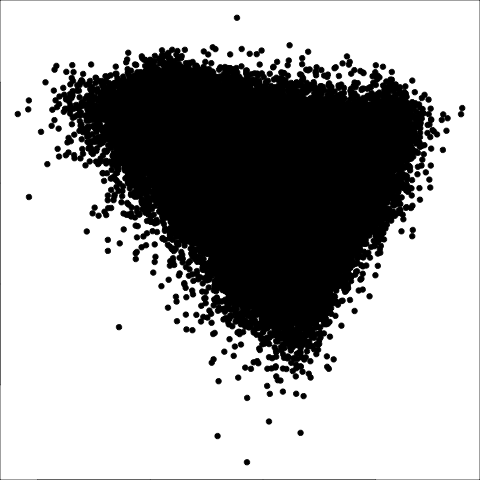
\includegraphics[width = 0.2\textwidth]{figures/vowels.png}} \\
	\end{diagram}
	

\end{frame}

%% Motivation:
%%	Classical / Laboratory Phonology
%%	Naturalistic language observation is also useful / crucial\

%% Outline:
%%	Establish a linking hypothesis between observable phonetic variation and phonological structure
%%		Universal Phonetics vs. Langauge Specific Phonetics vs. Exemplar Theory
%%	Case Study

\section{Phonology-Phonetic Interface}

\begin{frame}{Phonology-Phonetic Interface}

	\begin{block}{Options}
		\begin{itemize}
			\item Universal Phonetic Implementation
			\item Langauge Specific Phonetic Implementation
			\item Exemplar Theory
		\end{itemize}
	\end{block}

\end{frame}

\begin{frame}{Phonology-Phonetic Interface}
	
	\begin{block}{Linking Hypothesis}
		All I have to work with is phonetic measurements, so settling on a PH-interface model
		is crucial in order to make any connection to phonological theory at all.
	\end{block}

\end{frame}

\subsection{Universal Phonetic Implementation}



\setkeys{Gin}{with = 0.8\textwidth}

\begin{frame}{Phonology-Phonetic Interface}
	\framesubtitle{Continuous Change}

\includegraphics{fruehwald_CLS_2011-002}
	
	
\end{frame}



\begin{frame}{Phonology-Phonetic Interface}
	\framesubtitle{Continuous Change}

\includegraphics{fruehwald_CLS_2011-004}
	
	
\end{frame}

\begin{frame}{Phonology-Phonetic Interface}

	\begin{block}{Options}
		\begin{itemize}
			\item \sout{Universal Phonetic Implementation}
			\item Langauge Specific Phonetic Implementation
			\item Exemplar Theory
		\end{itemize}
	\end{block}

\end{frame}

\subsection{Exemplar Theory}




\setkeys{Gin}{width = 0.32\textwidth}

\begin{frame}{Phonology-Phonetic Interface}
	\framesubtitle{Category Shifts}
\begin{figure}
\includegraphics{fruehwald_CLS_2011-007}
\includegraphics{fruehwald_CLS_2011-008}
\includegraphics{fruehwald_CLS_2011-009}


\end{figure}
\end{frame}


\setkeys{Gin}{width = 0.8\textwidth}


\begin{frame}{Phonology-Phonetic Interface}
	\framesubtitle{Category Shifts}
\begin{block}{Canadian Shift}
	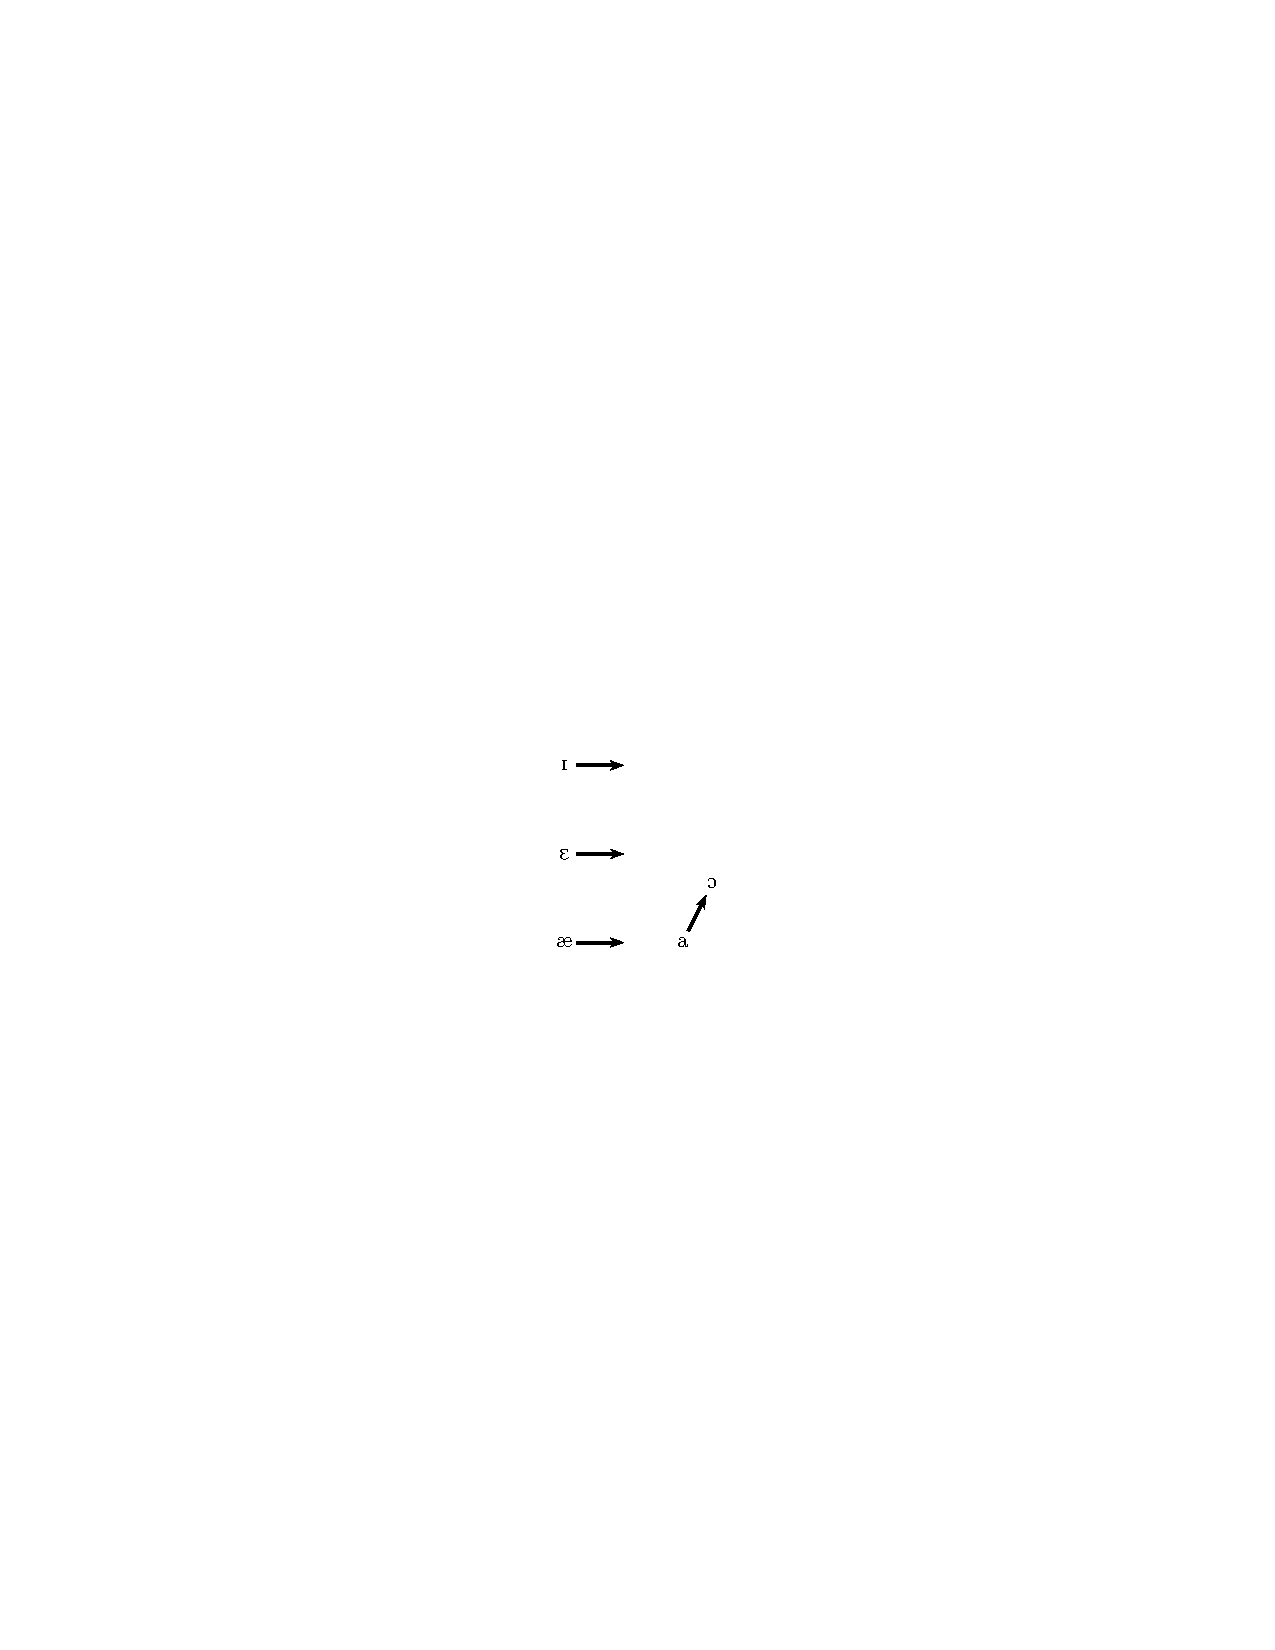
\includegraphics[width = 0.25\textwidth]{figures/canshift.pdf}
\end{block}
\end{frame}


\begin{frame}{Phonology-Phonetic Interface}
	\framesubtitle{Category Correlation}
	
	\begin{block}{Correlation of Philadelphia Vowels}
		\begin{itemize}
			\item For the vowel means for each speaker, I calculated the correlations for every pairwise vowel
			comparison across speakers, once for F1, once for F2.
			\item For each pairwise comparison, I also coded for whether the two vowels also 
			shared phonological specifications for height (3 degrees) or backness (2 degrees).
		\end{itemize}
	\end{block}
\end{frame}




\setkeys{Gin}{width = 1\textwidth}

\begin{frame}{Phonology-Phonetic Interface}
	\framesubtitle{Category Correlation}
\includegraphics{fruehwald_CLS_2011-012}
\end{frame}


\setkeys{Gin}{width = 0.8\textwidth}


\begin{frame}{Phonology-Phonetic Interface}
	\framesubtitle{Category Correlation}
	
	\begin{block}{Correlation of Philadelphia Vowels}
		\begin{itemize}
			\item This result is suggestive that inter-speaker phonetic variation (due to change or any other reason) is relatable
					to phonological features, not just atomic phonemes.
			\item May also be used as a phonological diagnostic.
				\begin{itemize}
					\item The above analysis categorized /ow/ and /uw/ as [$-$back], since they are undergoing a change of fronting.
					\item What would it look like of they were categorized as [$+$back]?
				\end{itemize}
		\end{itemize}
	\end{block}

\end{frame}






\setkeys{Gin}{width = 0.8\textwidth}

\begin{frame}{Phonology-Phonetic Interface}
	\framesubtitle{Category Correlation}
\includegraphics{fruehwald_CLS_2011-015}

\end{frame}




\subsection{Language Specific Phonetics}
\begin{frame}{Phonology-Phonetic Interface}

	\begin{block}{Options}
		\begin{itemize}
			\item \sout{Universal Phonetic Implementation}
			\item Langauge Specific Phonetic Implementation
			\item \sout{Exemplar Theory}
		\end{itemize}
	\end{block}

\end{frame}

\begin{frame}{Phonology-Phonetic Interface}
\begin{diagram}
\fbox{Phonology} & \mbox{uw} \rightarrow \mbox{[+back]/\underline{\hskip 15pt}l}  \\
\dTo & \\
\fbox{Language Specific Implementation} & \mbox{[+back]} \rightarrow 3\mbox{ on F2}\\
\dTo & \\
\fbox{Phonetic Alignment} & \mbox{\textipa{t\~{u:}n}}
\end{diagram}

\end{frame}

\begin{frame}{Phonology-Phonetic Interface}

	\begin{block}{In phonetic change...}
		\begin{itemize}
			\item The phonological representation remains stable (ish).
			\item The phonetic implementation of the phonological representation changes.
		\end{itemize}
	\end{block}
\end{frame}




\section{Identifying Phonological Processes}

\subsection{Utilizing Data on Phonetic Change}

\begin{frame}{Identifying Phonological Processes}

	\begin{block}{Follow}
		\begin{itemize}
			\item Phonological Unity $\rightarrow$ Phonetic Unity
			\item $\neg$Phonetic Unity $\rightarrow$ $\neg$Phonological Unity
		\end{itemize}
	\end{block}
	
	\begin{block}{Don't follow (but likely)}
		\begin{itemize}
			\item [*] Phonetic Unity $\rightarrow$ Phonological Unity
			\item [*] $\neg$Phonological Unity $\rightarrow$ $\neg$Phonetic Unity
		\end{itemize}
	\end{block}
\end{frame}



\subsection{Philadelphia /ey/}

\begin{frame}{Philadelphia /ey/}
	\framesubtitle{Past description}

			\begin{itemize}
				\item The peripheralization of /ey/ in non-word-final contexts was identified as
						a new and vigorous change in progress.
				\item The primary distinction that has been made is word final /ey/ versus other.
					\begin{itemize}
						\item {\it pay} [\textipa{pEI}]
						\item {\it make} [\textipa{m\|'eik}]
					\end{itemize}
			\end{itemize}
\end{frame}





\setkeys{Gin}{width = 1\textwidth}

\begin{frame}{Philadelphia /ey/}
	\framesubtitle{Past Description}
	
	\begin{columns}[c]
		\column{0.49\textwidth}
		
\alt<2>{
\includegraphics{fruehwald_CLS_2011-018}
}{
\includegraphics{fruehwald_CLS_2011-019}
}		
		
		\column{0.49\textwidth}
			\begin{block}{Questions}
				\begin{itemize}
					\item Are any other syllabic structures relevant?
					\item Are there any other phonological effects?
					\item How does it interact with morphology? (i.e.\ How does {\it pays} behave?)
				\end{itemize}
			\end{block}
	\end{columns}
\end{frame}


\setkeys{Gin}{width = 0.8\textwidth}


\begin{frame}{Philadelphia /ey/}
	\framesubtitle{Coding}
	
			\begin{itemize}
				\item 4 syllable types
					\begin{enumerate}
						\item Open
						\item Closed
						\item Final
						\item Hiatus
					\end{enumerate}
				\item Surface and ``Underlying'' Syllabification
				\item 5 Morphological Contexts
					\begin{enumerate}
						\item Null {\it pay}
						\item Inflectional {\it pays}
						\item Derivational {\it payment}
						\item Compounding  {\it paycheck}
						\item Contraction  {\it they'd}
					\end{enumerate}
			\end{itemize}
\end{frame}


\begin{frame}{Philadelphia /ey/}

\begin{tabular}{llllll}
\toprule
	&&\multicolumn{4}{c}{Underlying}\\
	
								&&Closed & Open & Hiatus & Final\\
	\cmidrule{3-6}
	\multirow{4}{*}{Surface}&Closed&{\it came} & -- & -- & {\it days}\\
						&Open	&{\it later} & {\it neighborhood} & -- & {\it playground}\\
						&Hiatus & -- & -- & {\it mayor} & {\it saying}\\
						&Final & -- & -- & -- & {\it they}\\
	\bottomrule
\end{tabular}


\end{frame}



\begin{frame}{Philadelphia /ey/}
	\framesubtitle{Syllabic Context}
First, only words with the same surface and ``underlying'' syllabification.

\includegraphics{fruehwald_CLS_2011-021}
	
\end{frame}

\begin{frame}{Philadelphia /ey/}
	\framesubtitle{Syllable Results}
	\begin{itemize}
		\item [] formula: \texttt{\footnotesize Diag $\sim$ (DOB/10) * Syllable + (Syllable | Speaker)}
		\item [] reference level: closed
	\end{itemize}
	\begin{columns}[c]
		\column{0.49\paperwidth}
	\begin{tabular}{rrr}
		\toprule
		&Estimate & t-value\\
	\cmidrule{2-3}
	Intercept & 0.57 & 11.1\\
	DOB 	  & 0.11 & 12.6\\
	\midrule
	open	  & -0.14 & -2.9\\
	final     & -0.04 & -0.7\\
	hiatus    & -0.21 & -0.6\\
	\midrule
	DOB$\times$ open &  0.02 & 2.9\\
	DOB$\times$ final & -0.08 & -9.1\\
	DOB$\times$ hiatus & -0.16 & -2.6\\
	\bottomrule
	\end{tabular}
		\column{0.49\paperwidth}
		\begin{block}{Slope Estimates}
			\begin{tabular}{lr@{=}l}
				closed & 0.11 & 0.11\\
				open & 0.13 & (0.11 + 0.02) \\
				final & 0.03 & (0.11 - 0.08) \\
				hiatus & -0.05 & (0.11 - 0.16)
			\end{tabular}
		\end{block}
	\end{columns}
\end{frame}


\begin{frame}{Phonology-Phonetic Interface}
	\framesubtitle{Segmental Context}

Following segment for closed and open syllables.
\includegraphics{fruehwald_CLS_2011-023}
		
\end{frame}


\begin{frame}{Philadelphia /ey/}
	\framesubtitle{Manner Results}
	\begin{itemize}
		\item [] formula: \texttt{\footnotesize Diag $\sim$ (DOB/10) * Manner + (Manner | Speaker)}
		\item [] reference level: stop
	\end{itemize}
	\begin{columns}[c]
		\column{0.49\paperwidth}
	\begin{tabular}{rrr}
		\toprule
		&Estimate & t-value\\
	\cmidrule{2-3}
	Intercept & 0.56 & 10.9\\
	DOB 	  & 0.11 & 13.2\\
	\midrule
	fricative & -0.08 & -1.3\\
	nasal     & -0.03 & -0.5\\
	lateral   & 0.38  & 2.8\\
	\midrule
	DOB$\times$fricative & 0.02 & 1.5\\
	DOB$\times$nasal     & 0.00 & 0.2\\
	DOB$\times$lateral   & -0.09 & -3.8\\
	\bottomrule
	\end{tabular}
		\column{0.49\paperwidth}
		\begin{block}{Slope Estimates}
			\begin{tabular}{lr@{=}l}
				stop & 0.11 & 0.11\\
				fricative & 0.13 & (0.11 + 0.02) \\
				nasal & 0.11 & (0.11 + 0.00) \\
				lateral & 0.02 & (0.11 - 0.09)
			\end{tabular}
		\end{block}
	\end{columns}
\end{frame}





\begin{frame}{Philadelphia /ey/}
	\framesubtitle{Interim Description}
	
	\begin{columns}[c]
		\column{0.49\textwidth}
		\begin{tabular}{ll}
			Non-undergoers & Undergoers\\
			\midrule
			Word-final & Everything Else\\
			Pre-hiatus & \\
			Pre-/l/ &
			\end{tabular}
		\column{0.49\textwidth}
		\begin{block}{Options}
			\begin{itemize}
				\item Undergoers and Non-undergoers are phonemically distinct.
				\item There is an active phonological process which differentiates undergoes and non-undergoers.
			\end{itemize}
		\end{block}
	\end{columns}
	
\end{frame}

\begin{frame}{Philadelphia /ey/}
	\framesubtitle{Morphological Interaction}

What effect does inflectional morphology have on otherwise word final /ey/?

\includegraphics{fruehwald_CLS_2011-026}
		
\end{frame}

\begin{frame}{Philadelphia /ey/}
	\framesubtitle{Morphological Results}
	\begin{itemize}
		\item [] formula: \texttt{\footnotesize Diag $\sim$ (DOB/10) * Morphology + (Morphology | Speaker)}
		\item [] reference level: Null
	\end{itemize}
	\begin{columns}[c]
		\column{0.49\paperwidth}
	\begin{tabular}{rrr}
		\toprule
		&Estimate & t-value\\
	\cmidrule{2-3}
	Intercept & 0.52 & 12.2\\
	DOB 	  & 0.03 & 4.2\\
	\midrule
	-ed & -0.09 & -0.8 \\
	-s  & -0.12 & -1.3\\
	-ing & -0.46 & -3.7\\
	\midrule
	DOB$\times$-ed & 0.05 & 2.7\\
	DOB$\times$-s     & 0.11 & 6.8\\
	DOB$\times$-ing   & -0.04 & -2.2\\
	\bottomrule
	\end{tabular}
		\column{0.49\paperwidth}
		\begin{block}{Slope Estimates}
			\begin{tabular}{lr@{=}l}
				final &  0.03 &  0.03\\
				-ed & 0.08 & (0.03 + 0.05) \\
				-s & 0.15 & (0.03 + 0.02) \\
				-ing & -0.01 & (0.03 - 0.04)
			\end{tabular}
		\end{block}
	\end{columns}
\end{frame}



\begin{frame}{Philadelphia /ey/}
	\framesubtitle{Final Pattern}
All unaffixed, or affixed inflectional morphology in 4 contexts: Word-final, Pre-hiatus, Pre-l, and elsewhere.
\includegraphics{fruehwald_CLS_2011-028}
		
\end{frame}

\begin{frame}{Philadelphia /ey/}
	\framesubtitle{Phonological Description}
	
	\begin{block}{Phonological Process}
		ey $\rightarrow$ [+peripheral]/\underline{\hskip 15pt}C\ldots]$_{word}$
	\end{block}
	
	\begin{block}{Phonetic Change}
		\begin{enumerate}
			\item ey$_{+periph}$ $\rightarrow$ 0.1 peripherality
			\item ey$_{+periph}$ $\rightarrow$ 0.2 peripherality
			\item \ldots
		\end{enumerate}
	\end{block}
	
	\begin{block}{Phonetic Alignment}
		\begin{itemize}
			\item {[}eyl] $\rightarrow$ more peripheral
			\item {[}ey\#] $\rightarrow$ less peripheral
		\end{itemize}
	\end{block}
\end{frame}

\begin{frame}{Philadelphia /ey/}
	\framesubtitle{Phonological Description}
	
	\begin{block}{Phonological Process}
		ey $\rightarrow$ [+peripheral]/\underline{\hskip 15pt}C\ldots]$_{word}$
	\end{block}
	\begin{block}{/l/ is not a C?}
		\begin{itemize}
			\item /l/ undergoes extreme vocalization in Philadelphia.
				\begin{itemize}
					\item Intervocalically ({\it balance})
					\item Initial Clusters ({\it floor})
				\end{itemize}
			\item Triggers offglide deletion in /aw/.
				\begin{itemize}
					\item {\it Powel} = {\it pal}
				\end{itemize}
		\end{itemize}
		
	\end{block}
\end{frame}




\subsection{The Unique View of Diachrony}



\begin{frame}{The Unique View of Diachrony}
	Would a study without a view of the changing state of the speech community have come
	to the same conclusions?

\end{frame}

\begin{frame}{The Unique View of Diachrony}
	If you had done a study of college aged Philadelphians in 2002, this is what you would have seen.
	
\includegraphics{fruehwald_CLS_2011-030}
\end{frame}


\begin{frame}{The Unique View of Diachrony}
If you had done a study of Philadelphians aged 18 to 70 in 2002, this is what you would have seen.
	
\includegraphics{fruehwald_CLS_2011-032}
\end{frame}



\section{Conclusion}





\end{document}  
